\documentclass{article}

\usepackage{fancyhdr}
\usepackage{extramarks}
\usepackage{amsmath}
\usepackage{amsthm}
\usepackage{amsfonts}
\usepackage{tikz}
\usepackage[plain]{algorithm}
\usepackage{algpseudocode}
\usepackage{xcolor}
\usepackage{enumitem}
\usepackage{amssymb}
\usepackage{todonotes}
\usepackage{mathtools}
\usepackage{wasysym}
\usepackage{cancel}
\usepackage{phaistos}
\usepackage[usestackEOL]{stackengine}[2013-10-15]
\def\x{\hspace{6ex}}    %BETWEEN TWO 1-DIGIT NUMBERS
\def\y{\hspace{4.9ex}}  %BETWEEN 1 AND 2 DIGIT NUMBERS
\def\z{\hspace{3.8ex}}    %BETWEEN TWO 2-DIGIT NUMBERS
\stackMath

\usetikzlibrary{automata,positioning}

%
% Basic Document Settings
%

\topmargin=-0.45in
\evensidemargin=0in
\oddsidemargin=0in
\textwidth=6.5in
\textheight=9.0in
\headsep=0.25in

\linespread{1.1}

\pagestyle{fancy}
\lhead{\hmwkAuthorName}
\chead{\hspace{2.5cm} \hmwkClass\ (\hmwkClassInstructor): \hmwkTitle}
\rhead{\firstxmark}
\lfoot{\lastxmark}
\cfoot{\thepage}

\renewcommand\headrulewidth{0.4pt}
\renewcommand\footrulewidth{0.4pt}

\setlength\parindent{0pt}

%
% Create Problem Sections
%

\newcommand{\enterProblemHeader}[1]{
    \nobreak\extramarks{}{Problem \arabic{#1} continued on next page\ldots}\nobreak{}
    \nobreak\extramarks{Problem \arabic{#1} (continued)}{Problem \arabic{#1} continued on next page\ldots}\nobreak{}
}

\newcommand{\exitProblemHeader}[1]{
    \nobreak\extramarks{Problem \arabic{#1}}{Problem \arabic{#1} continued on next page\ldots}\nobreak{}
    \stepcounter{#1}
    \nobreak\extramarks{Problem \arabic{#1}}{}\nobreak{}
}

\newcount\colveccount
\newcommand*\colvec[1]{
        \global\colveccount#1
        \begin{pmatrix}
        \colvecnext
}
\def\colvecnext#1{
        #1
        \global\advance\colveccount-1
        \ifnum\colveccount>0
                \\
                \expandafter\colvecnext
        \else
                \end{pmatrix}
        \fi
}

\setcounter{secnumdepth}{0}
\newcounter{partCounter}
\newcounter{homeworkProblemCounter}
\setcounter{homeworkProblemCounter}{1}
\nobreak\extramarks{Problem \arabic{homeworkProblemCounter}}{}\nobreak{}

%
% Homework Problem Environment
%
% This environment takes an optional argument. When given, it will adjust the
% problem counter. This is useful for when the problems given for your
% assignment aren't sequential. See the last 3 problems of this template for an
% example.
%
\newenvironment{homeworkProblem}[1][-1]{
    \ifnum#1>0
        \setcounter{homeworkProblemCounter}{#1}
    \fi
    \section{Problem \arabic{homeworkProblemCounter}}
    \setcounter{partCounter}{1}
    \enterProblemHeader{homeworkProblemCounter}
}{
    \exitProblemHeader{homeworkProblemCounter}
}

%
% Homework Details
%   - Title
%   - Due date
%   - Class
%   - Section/Time
%   - Instructor
%   - Author
%

\newcommand{\hmwkTitle}{Assignment 4}
\newcommand{\hmwkDueDate}{October 28, 2018}
\newcommand{\hmwkClass}{Probability \& Statistics}
\newcommand{\hmwkClassTime}{Fall Semester}
\newcommand{\hmwkClassInstructor}{Prof. D. Eynard}
\newcommand{\hmwkAuthorName}{\textbf{A. Romanelli} / \textbf{A. Vicini}}

%
% Title Page
%

\title{
    \vspace{2in}
    \textmd{\textbf{\hmwkClass:\ \hmwkTitle}}\\
    \normalsize\vspace{0.1in}\small{Due\ on\ \hmwkDueDate\ at 8:30am}\\
    \vspace{0.1in}\large{\textit{\hmwkClassInstructor}}
    \vspace{3in}
}

\author{\hmwkAuthorName}
\date{}

\renewcommand{\part}[1]{\textbf{\large Part \Alph{partCounter}}\stepcounter{partCounter}\\}

%
% Various Helper Commands
%

% Useful for algorithms
\newcommand{\alg}[1]{\textsc{\bfseries \footnotesize #1}}

% For derivatives
\newcommand{\deriv}[1]{\frac{\mathrm{d}}{\mathrm{d}x} (#1)}

% For partial derivatives
\newcommand{\pderiv}[2]{\frac{\partial}{\partial #1} (#2)}

% Integral dx
\newcommand{\dx}{\mathrm{d}x}

% Alias for the Solution section header
\newcommand{\solution}{\textbf{\large Solution}}

% Probability commands: Expectation, Variance, Covariance, Bias
\newcommand{\E}{\mathrm{E}}
\newcommand{\Var}{\mathrm{Var}}
\newcommand{\Cov}{\mathrm{Cov}}
\newcommand{\Bias}{\mathrm{Bias}}

\begin{document}

\maketitle

\pagebreak

\begin{homeworkProblem}
	We let $n$ be the number of steps taken and draw the Pascal's Triangle:
	\begin{center}
			\Longstack[l]{
			n=0\\
			n=1\\
			n=2\\
			n=3\\
			n=4\\
			n=5\\
			n=6\qquad\ \\
			}
			\Longstack{
			1\\
			1\x 1\\
			1\x 2\x 1\\
			1\x 3\x 3\x 1\\
			1\x 4\x 6\x 4\x 1\\
			1\x 5\y 10\z 10\y 5\x 1\\
			1\x 6\y 15\z 20\z 15\y 6\x 1\\
			}
	\end{center}

	\begin{enumerate}[label=\textbf{\alph*)}]
		\item There's no possible way with a random walk of odd length to return to the origin.
		\item $\binom64\cdot\frac1{2^{6}} = \frac{15}{64}$
		\item There's no random walk which reaches a distance of 6 in only 4 steps.
		\item $\binom53\cdot\frac1{2^5} = \frac{5}{16}$
		\item In the considered set of possible steps, our prime numbers are: $\{2,3,5\}$, thus our chance is:
		$$P_{S_6}(\text{primes}) = P_{S_6}(\text{2D4U}) + P_{S_6}(\text{3D3U}) + P_{S_6}(\text{5D1U}) = $$ 
		$$P_{S_6}(2) = P_{S_6}(2) + P_{S_6}(0) + P_{S_6}(-4) = \frac1{64}\cdot\binom61 + \frac1{64}\cdot\binom63 + \frac1{64}\cdot\binom64 = \frac6{64} + \frac{20}{64} + \frac{15}{64} = \frac{41}{64}$$ 
		\item Out of all the possible 64 combinations, we want to calculate what is the chance of having two upward movements in a row and then compute its complement.
		If we have less than two moves down, then we know for sure that the path will contain at least two upward movement in a row, we compute how many combinations:
		$$2^6\cdot P(0D6U) = \binom66 = 1, \qquad 2^6\cdot P(1D5U) = \binom65 = 6, \qquad 2^6\cdot P(2D4U) = \binom64 = 15$$
		In the case of $P(3D3U)$ we'll need to enumerate the cases in which we DON'T have two upward movements in a row:
		\begin{itemize}
			\item UDUDUD
			\item DUDUDU
			\item UDDUDU
			\item UDUDDU
		\end{itemize}
		Thus we take these four cases out of our calculations: $$2^6\cdot P(3D3U) - 4 = \binom63 - 4 = 20 - 4 = 16$$
		In the last scenario of $P(4D2U)$ we only have five possible chances:
		\begin{itemize}
			\item UUDDDD
			\item DUUDDD
			\item DDUUDD
			\item DDDUUD
			\item DDDDUU
		\end{itemize}
		We can finally sum all of the possible outcomes which involve a sequence of two upward movements in a row that we computed so far: $2^6\cdot P(2U\text{ in a row}) = 1 + 6 + 15 + 16 + 5 = 43$
		Now we calculate the complement of what we just computed: $1 - \frac{43}{64} = \frac{21}{64} = P(\text{not 2U in a row})$
	\end{enumerate}
\end{homeworkProblem}
\begin{homeworkProblem}
	Initially, out of all the possible scenarios, only $\frac34$ will end with at least one of the two teams successfully completing their project. Thus we get the following table:
	\begin{table}[h]
		\centering
		\begin{tabular}{c|cc|c}
			& A = S & A = F & P(B) \\
			\hline
			B = S & & & $\frac12$ \\
			B = F & & $\frac14$ & \\
			\hline
			P(A) & $\frac23$ & & \\
		\end{tabular}
	\end{table} \\ 
	With our partially filled table, we can still deduce some additional data, considering the fact that the marginals must sum up to 1:
	\begin{table}[h]
		\centering
		\begin{tabular}{c|cc|c}
			& A = S & A = F & P(B) \\
			\hline
			B = S & & & $\frac12$ \\
			B = F & & $\frac14$ & $\frac12$ \\
			\hline
			P(A) & $\frac23$ & $\frac13$ & \\
		\end{tabular}
	\end{table}
	Moreover, we can deduce $P(A = F, B = S) = P(A = F) - P(A = F, B = F)$:
	\begin{table}[h]
		\centering
		\begin{tabular}{c|cc|c}
			& A = S & A = F & P(B) \\
			\hline
			B = S & $\frac5{12}$ & $\frac1{12}$ & $\frac12$ \\
			B = F & $\frac14$ & $\frac14$ & $\frac12$ \\
			\hline
			P(A) & $\frac23$ & $\frac13$ & \\
		\end{tabular}
	\end{table} \\ 
	This table now allows us to look up the probability of the considered event $P(A = F, B = S) = \frac1{12}$
	\begin{center}
		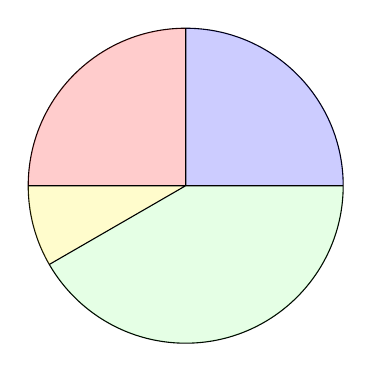
\begin{tikzpicture}
			\draw (0,0) circle (2cm);
			\fill[red,opacity=0.2] (-2,0) -- ++(0:2) -- +(90:2) -- (0,2) arc (90:180:2) -- cycle;
			\fill[blue, opacity=0.2] (0,2) -- ++(270:2) -- +(0:2) -- (2,0) arc (180:270:-2) -- cycle;
			\fill[yellow, opacity=0.2] (0,0) -- ++(180:2) -- (-2,0) arc (180:210:2) -- cycle;
			\fill[green, opacity=0.1] (0,0) -- ++(0:2) -- (2,0) arc (180:30:-2) -- cycle;

			\draw (-2, 0) -- (0,0) -- (0, 2) -- (0,0) -- (2,0) -- (0,0) -- (-1.732, -1);

		\end{tikzpicture}
		\hspace{0.5cm}
		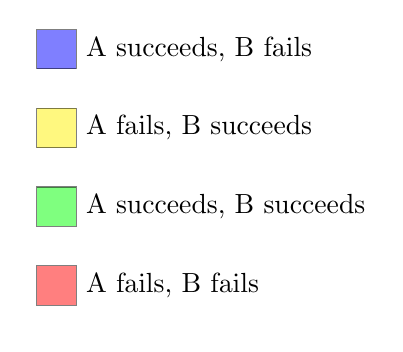
\begin{tikzpicture}
			\fill[red, opacity=0.5, draw=black] (0,0) rectangle (0.5,0.5);
			\node[right] at (0.5,0.25) {A fails, B fails};
			\fill[green, opacity=0.5, draw=black] (0,1) rectangle (0.5,1.5);
			\node[right] at (0.5,1.25) {A succeeds, B succeeds};
			\fill[yellow, opacity=0.5, draw=black] (0,2) rectangle (0.5,2.5);
			\node[right] at (0.5,2.25) {A fails, B succeeds};
			\fill[blue, opacity=0.5, draw=black] (0,3) rectangle (0.5,3.5);
			\node[right] at (0.5,3.25) {A succeeds, B fails};
			\node at (0, -0.125) {};
		\end{tikzpicture} 
		\hspace{0.5cm}
%		\begin{figure}[!h]
			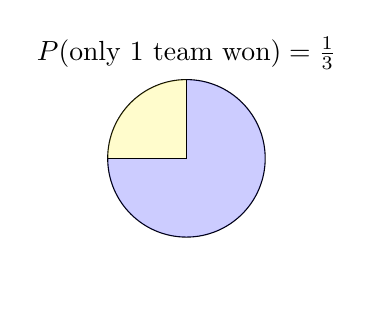
\begin{tikzpicture}[scale=0.5]
				\draw (0,0) circle (2cm);
				\fill[yellow,opacity=0.2] (-2,0) -- ++(0:2) -- +(90:2) -- (0,2) arc (90:180:2) -- cycle;
				\fill[blue, opacity=0.2] (0,0) -- ++(90:2) -- (0,2) arc (270:0:-2) -- cycle;
	%			\fill[yellow, opacity=0.2] (0,0) -- ++(180:2) -- (-2,0) arc (180:210:2) -- cycle;
	%			\fill[green, opacity=0.1] (0,0) -- ++(0:2) -- (2,0) arc (180:30:-2) -- cycle;
				\draw (-2, 0) -- (0,0) -- (0, 2);
				\node[above] at (0, 2) {$P(\text{only 1 team won}) = \frac13$};
				\node at (0,-3.5) {};
			\end{tikzpicture}
%		\end{figure} 
		
		\vspace{0.5cm}
%		We can see it that representing the exercise as a pie chart the solution is immediately intuitive: the chance that only B succeeds, is given by the total, minus the failure chance, minus the chance of winning of A. Which gives $1 - \frac14 - \frac23 = \frac1{12}$
	\end{center}
	But if we now know for a fact that only one team did succeed and we must compute the chance of team B being the one successful, then we need to consider how many scenarios were having only one team being successful (in the pie chart yellow+blue). \\ \\
	We can use the formula to compute the conditional probability:
	$$\hspace{-1cm}P(B = S|\text{1 team won}) = \frac{P((B = S) \cap (\text{only 1 team won}))}{P(\text{only 1 team won})} =  \frac{P(A = F, B = S)}{P(A = F, B = S) + P(A = S, B = F)} = \frac{\frac1{12}}{\frac13} = \frac3{12} = \frac14$$
	Which is the probability that, given that one team has won, B was the one being successful.
\end{homeworkProblem}
\newpage\begin{homeworkProblem}
	\begin{enumerate}[label=\textbf{\alph*)}]
		\item $P_Y(Y=16) = 0.08 + 0.28 + 0.04 =0.4$
		\item $P_X = \{0.12+0.08, 0.42+0.28, 0.06+0.04\} \Rightarrow P_X = \{0.2, 0.7, 0.1\}$
		\item According to \textbf{Definition 12}, $P_X(130)$ and $P_Y(16)$ are statistically independent because: $$P(P(X = 130) \cap P(Y = 16)) = P_X(130) \cdot P_Y(16)$$
		$$0.28 = 0.7 \cdot 0.4 \implies \textbf{true}$$
		\item We can show that $X$ and $Y$ are independent if we show what we demonstrated at point \textbf{c)} for each event.
		\begin{table}[h]
			\centering
			\begin{tabular}{ccc|cccc}
				&&&&X&& \\
				&&&0.2&0.7&0.1 \\
				&&&129&130&131 \\
				\hline
				Y&0.6&15&$0.2\cdot0.6$&$0.7\cdot0.6$&$0.1\cdot0.6$\\
				 &0.4&16&$0.2\cdot0.4$&$0.7\cdot0.4$&$0.1\cdot0.4$
			\end{tabular}
			\hspace{2cm}
			\begin{tabular}{cc|cccc}
				&&&X&& \\
				&&129&130&131 \\
				\hline
				Y&15&0.12&0.42&0.06\\
				 &16&0.08&0.28&0.04
			\end{tabular}		
		\end{table}
	\end{enumerate}
\end{homeworkProblem}
\newpage\begin{homeworkProblem}
	We apply Bayes' Theorem to compute the following probabilities:
	$$P(B|A) = \frac{P(B) \cdot P(A|B)}{P(A|B)\cdot P(B) + P(A|B^C)(1-P(B))}$$
	\begin{enumerate}[label=\textbf{\alph*)}]
		\item $$P(\text{SPAM}|\text{shoes}) = \frac{P(\text{SPAM}) \cdot P(\text{shoes}|\text{SPAM})}{ P(\text{shoes}|\text{SPAM}) \cdot P(\text{SPAM}) + P(\text{shoes}|\text{SPAM}^C)(1 - P(\text{SPAM}))} =$$
		$$= \frac{\frac12 \cdot \frac1{16}}{\frac{1}{16} \cdot \frac12 + \frac{2}{14} \cdot \frac12} = \frac{\frac{1}{32}}{\frac{1}{32} + \frac{1}{14}} = \frac{\frac1{32}}{\frac{23}{224}} = \frac{224}{736} = \frac7{23}$$
		\item $$P(\text{SPAM}|\text{walk}\cup\text{zoo}) = \frac{P(\text{SPAM}) \cdot P(\text{SPAM}|\text{walk}\cup\text{zoo})}{ P(\text{walk}\cup\text{zoo}|\text{SPAM}) \cdot P(\text{SPAM}) + P(\text{walk}\cup\text{zoo}|\text{SPAM}^C)(1 - P(\text{SPAM}))} =$$
		$$= \frac{\frac12 \cdot \frac0{16}}{\frac0{16} \cdot \frac12 + \frac{4}{14} \cdot \frac12} = 0$$
		\item $$P(\text{SPAM}|\text{free}\cap\text{deal}) = \frac{P(\text{SPAM}) \cdot P(\text{SPAM}|\text{free}\cap\text{deal})}{ P(\text{free}\cap\text{deal}|\text{SPAM}) \cdot P(\text{SPAM}) + P(\text{free}\cap\text{deal}|\text{SPAM}^C)(1 - P(\text{SPAM}))} =$$
		$$= \frac{\frac12 \cdot \frac2{16}}{\frac2{16} \cdot \frac12 + \frac0{14} \cdot \frac12} = \frac{\frac1{16}}{\frac1{16}} = 1$$
		\item $$P(\text{SPAM}|\text{puma}\cup\text{giraffe}) = \frac{P(\text{SPAM}) \cdot P(\text{SPAM}|\text{puma}\cup\text{giraffe})}{ P(\text{puma}\cup\text{giraffe}|\text{SPAM}) \cdot P(\text{SPAM}) + P(\text{puma}\cup\text{giraffe}|\text{SPAM}^C)(1 - P(\text{SPAM}))} =$$
		$$= \frac{\frac12 \cdot \frac1{16}}{\frac1{16} \cdot \frac12 + \frac3{14} \cdot \frac12} = \frac{\frac1{32}}{\frac1{32} + \frac3{28}} = \frac{\frac1{32}}{\frac{31}{224}} = \frac{224}{992} = \frac{7}{31} $$	\end{enumerate}
\end{homeworkProblem}
\newpage
\section{Optional Problem}
\end{document}
